\chapter{Opis ostatecznego rozwiązania}
\thispagestyle{chapterBeginStyle}

\section{Wizualizacja rozwiązania}

\begin{figure}[htbp]
    \centering
    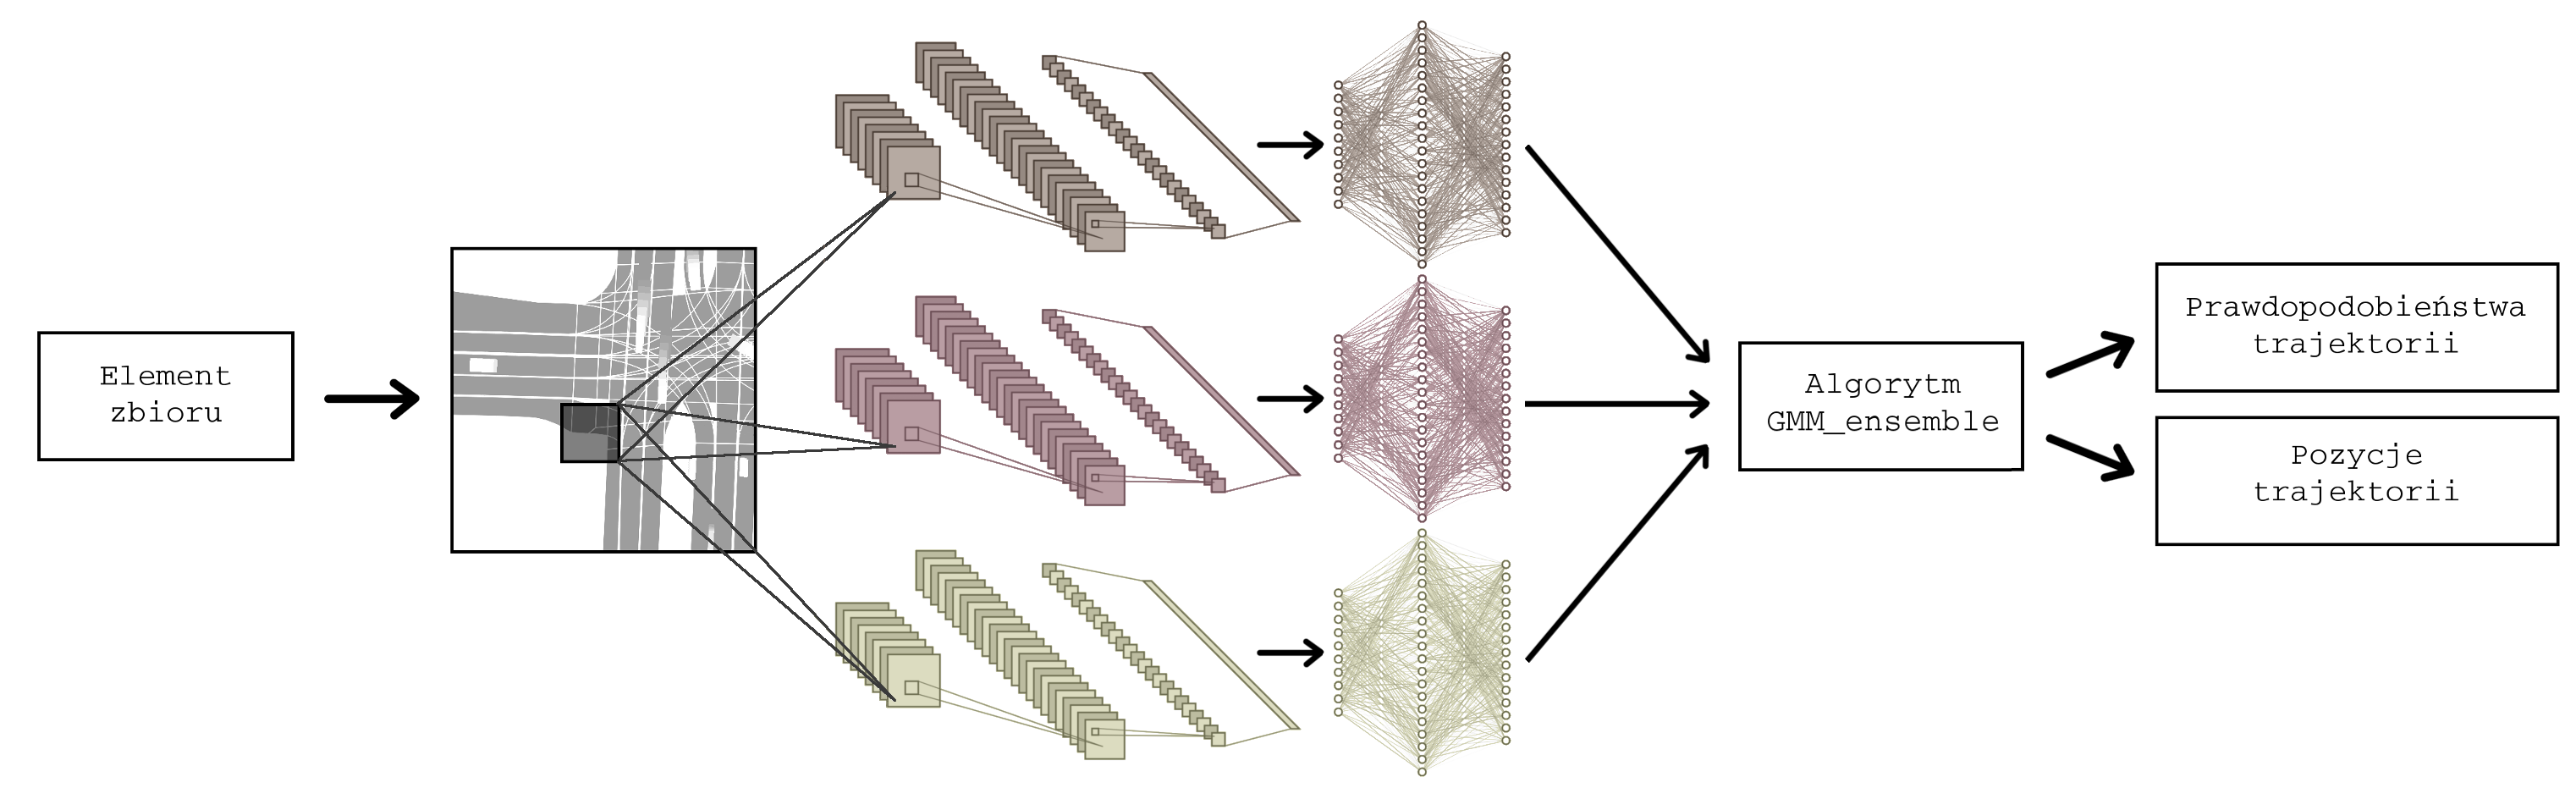
\includegraphics[width=\linewidth]{nn_schema_ensemble.png}
    \caption{Wizualizacja architektury finalnego rozwiązania}
\end{figure}

\section{Opis rozwiązania}
Rozwiązanie, które okazało się najlepsze spośród wszystkich rozważanych w tej pracy to model składający się z trzech sieci neuronowych o architekturach szkieletów \texttt{ResNet-18}, \texttt{MixNet-M}, \texttt{MixNet-L}. Modele te trenowane były z użyciem rasteryzatora \texttt{SemBoxRasterizer} (ten rasteryzator powinien być również wykorzystywany do przewidywania na danych spoza rozważanego zbioru np. w środowisku produkcyjnym). Do agregacji predykcji wykorzystano mieszaninę rozkładów Gaussa, która pozwala na uzyskanie trzech najbardziej prawdopodobnych trajektorii. Model składający się z wcześniej opisanych trzech sieci konwolucyjnych oraz agregacji predykcji posiada uśrednioną wartość funkcji kosztu równą 11.05 (na zbiorze testowym). Jest to bardzo dobry wynik, który można porównać do wartości funkcji kosztu na wizualizacjach w rozdziale 5. Osiągnięty rezultat jest bardzo bliski rozwiązaniom SOTA (ang. state of the art) na wykorzystanym zbiorze danych. Uzyskany model wykorzystuje obliczenia równoległe, dzięki czemu przy wykorzystaniu trzech jednostek GPU, czas jaki jest potrzebny do wykonania predykcji maleje około 3 razy w porównaniu z predykcją na jednej jednostce GPU. Wykonanie jednej predykcji na uzyskanym modelu z trzema jednostkami GPU jest bardzo szybkie, zajmuje około 10ms.